% chktex-file 19
\documentclass[a4paper,14pt,oneside,openany]{memoir}
\usepackage{tempora}
\usepackage[russian]{babel}
\usepackage[utf8]{inputenc}
\usepackage{csquotes}
\usepackage{indentfirst}
\usepackage[bibstyle=gost-numeric,citestyle=gost-numeric]{biblatex}
\usepackage{geometry}
\usepackage[bigdelims,vvarbb]{newtxmath}
\usepackage{graphicx}
\usepackage{relsize}
\geometry{a4paper, top=20mm, bottom=20mm, left=25mm, right=15mm}
\DeclareBibliographyCategory{cited}
\AtEveryCitekey{\addtocategory{cited}{\thefield{entrykey}}}
\newtheorem{defn}{Определение}
\renewcommand{\baselinestretch}{1.5}

% Page numbering style
\makeevenhead{plain}{}{\thepage}{}
\makeoddhead{plain}{}{\thepage}{}
\makeevenfoot{plain}{}{}{}
\makeoddfoot{plain}{}{}{}
\pagestyle{plain}

% Headers etc.
\newcommand{\basegostsectionfont}{\fontsize{15pt}{17pt}\selectfont\bfseries}
\newcommand{\hdngalign}{\centering}
\newcommand{\hdngaligni}{}
\newlength{\myindentlen}
\setlength{\myindentlen}{1\parindent}

\newlength{\curtextsize}
\setlength{\myindentlen}{15pt}

\makechapterstyle{thesisgost}{%
    \chapterstyle{default}
    \setlength{\beforechapskip}{0pt}
    \setlength{\midchapskip}{0pt}
    \setlength{\afterchapskip}{3\curtextsize}
    \renewcommand*{\chapnamefont}{\basegostsectionfont}
    \renewcommand*{\chapnumfont}{\basegostsectionfont}
    \renewcommand*{\chaptitlefont}{\basegostsectionfont}
    \renewcommand*{\chapterheadstart}{}
    \renewcommand*{\afterchapternum}{.\space}
    \renewcommand*{\printchapternum}{\hdngaligni\hdngalign\chapnumfont \thechapter}
    \renewcommand*{\printchaptername}{}
    \renewcommand*{\printchapternonum}{\hdngaligni\hdngalign}
}

\makeatletter
\makechapterstyle{thesisgostchapname}{%
    \chapterstyle{thesisgost}
    \renewcommand*{\printchapternum}{\chapnumfont \thechapter}
    \renewcommand*{\printchaptername}{\hdngaligni\hdngalign\chapnamefont \@chapapp} %
}
\makeatother

\chapterstyle{thesisgost}

\setsecheadstyle{\basegostsectionfont\hdngalign}
\setsecindent{\myindentlen}

\setsubsecheadstyle{\basegostsectionfont\hdngalign}
\setsubsecindent{\myindentlen}

\setsubsubsecheadstyle{\basegostsectionfont\hdngalign}
\setsubsubsecindent{\myindentlen}

\sethangfrom{\noindent #1}

\chapterstyle{thesisgostchapname}
\renewcommand*{\cftchaptername}{\chaptername\space}

% \setbeforesecskip{3\curtextsize}
% \setaftersecskip{3\curtextsize}
% \setbeforesubsecskip{3\curtextsize}
% \setaftersubsecskip{3\curtextsize}
% \setbeforesubsubsecskip{3\curtextsize}
% \setaftersubsubsecskip{3\curtextsize}

\setlength{\cftbeforechapterskip}{0pt plus 0pt}
\renewcommand*{\insertchapterspace}{}

\bibliography{biblio}
\nocite{*}
%\DeclareUnicodeCharacter{0301}{*************************************}
\begin{document}
\relscale{1.07}
\sloppy
% Титульный лист (ГОСТ Р 7.0.11-2001, 5.1)
\thispagestyle{empty}
\begin{center}
    Казанский (Приволжский) федеральный университет
\end{center}
%
\vspace{0pt plus4fill} %число перед fill = кратность относительно некоторого расстояния fill, кусками которого заполнены пустые места
\begin{flushright}
    На правах рукописи

    %\textsl {УДК \thesisUdk}
\end{flushright}
%
\vspace{0pt plus6fill} %число перед fill = кратность относительно некоторого расстояния fill, кусками которого заполнены пустые места
\begin{center}
    {\large Д. Н. Галанин}
\end{center}
%
\vspace{0pt plus1fill} %число перед fill = кратность относительно некоторого расстояния fill, кусками которого заполнены пустые места
\begin{center}
    \textbf {\large %\MakeUppercase
        Разработка методов оценки релевантности результатов поиска в семантических поисковых системах}

    \vspace{0pt plus2fill} %число перед fill = кратность относительно некоторого расстояния fill, кусками которого заполнены пустые места
    {%\small
        Специальность 02.06.01\ "---

        <<Компьютерные и информационные науки>>
    }

    \vspace{0pt plus2fill} %число перед fill = кратность относительно некоторого расстояния fill, кусками которого заполнены пустые места
    Диссертация на соискание учёной степени

    кандидата наук
\end{center}
%
\vspace{0pt plus4fill} %число перед fill = кратность относительно некоторого расстояния fill, кусками которого заполнены пустые места
\begin{flushright}

    Научный руководитель:

    кандидат наук, доцент

    Н. Р. Бухараев

\end{flushright}
%
\vspace{0pt plus4fill} %число перед fill = кратность относительно некоторого расстояния fill, кусками которого заполнены пустые места
{\centering Казань\ "--- 2021\par}
\newpage
\tableofcontents
\chapter*{Введение}
\subsubsection{Актуальность темы исследования}
Проблемы информационного поиска в настоящее время представляют значительный интерес, как коммерческий, так и академический. Объемы обрабатываемой
и хранимой информации постоянно растут, в связи с чем остро стоят проблемы ее структурирования и каталогизации. В сети Интернет, без которой сейчас
уже невозможно представить существование современного мира, добыча и отбор нужной информации происходит практически исключительно средствами
информационного поиска.

Поскольку основной объем данных в сети Интернет относится к неструктурированной информации (например, в роли таковой выступают
публицистические и новостные статьи, аудио- и видеозаписи и т. д.), подавляющее большинство операций доступа к ней со стороны
простых пользователей выполняется с использованием информационно-поисковых систем. В частности, корпорация Alphabet, основным
продуктом которой является поисковая система Google, по состоянию на начало 2021 года занимает 4-е место на мировом рынке
ИТ-компаний с капитализацией в 1,22 триллиона долларов США \cite{forbestop100it}, что свидетельствует о наличии значительного
практического (коммерческого) интереса к сфере информационного поиска.

В то же время, например, поисковая система Bing, разработанная корпорацией Microsoft (2-е место в том же списке \cite{forbestop100it}),
в мире занимает 2-е место с более чем 13\% поисковых запросов, однако в России ее популярность невысока: менее 0,3\%, причем
на мобильных устройствах популярность ее более чем в 30 раз ниже, чем на компьютерах \cite{drmax2020} (где в большинстве
слкчаев предустановлена операционная система Windows, в которую встроена поддержка Bing). Связано это, прежде всего, с
недостаточной релевантностью поисковой выдачи Bing на русском языке (в отличие от английского), поэтому она сильно уступает
как Google, так и отечественной системе Yandex.

В связи со всем вышесказанным, существенную важность приобретает релевантность результатов поисковой выдачи, поскольку от нее напрямую зависит
качество применяемой поисковой системы, а также ее конкурентоспособность. Будучи мерой важности результатов выдачи поисковой системы для
ее пользователя --- человека, релевантность так или иначе является субъективной характеристикой. Однако же, очевидно, что она подлежит оценке
автоматизированными методами и алгоритмами.

Следовательно, мы можем говорить об актуальности проблемы оценки релевантности.

\subsubsection{Степень разработанности проблемы}
Проблемам ранжирования поиcковой выдачи посвящено большое количество научных работ и публикаций. Результаты подробного анализа
источников по теме исследования позволили сделать некоторые выводы:
\begin{enumerate}[1)]
    \item как правило, для оценки релевантности используются классические алгоритмы, причем большинство из них, в частности,
          широко известная функция BM25, были введены еще в 1970-х и 80-х годах (более современные модификации часто представляют
          собой вариации на базе существуовавших до этого методов);
    \item нейросетевые методы, используемые при ранжировании, например, широко известные алгоритмы класса trec\_eval
          \cite{10.1145/344250.344252}, часто представляют собой вероятностные методы;
    \item использование генеративно-состязательных сетей при ранжировании и оценке релевантности на текущий момент
          является довольно слабо разработанной областью в сфере информационного поиска. Генеративно-состязательные сети как понятие появились
          сравнительно недавно (середина 2010-х годов); они позволяют создавать объекты, в той или иной мере "<похожие"> на заданные.
          Данная концепция нашла свое применение для разнообразного спектра задач --- от генерации изображений и фотографий до
          применения в теории игр. Однако, в сфере информационного поиска описанный выше подход пока не получил широкого распространения,
          хотя он и упоминается в некоторых научных работах. Таким образом, следует считать необходимым проведение
          дальнейшего научного поиска в направлении нейросетевого подхода с использованием генеративно-состязательных сетей.
\end{enumerate}

\subsubsection{Цели и задачи исследования}


В связи с вышеизложенным, сформулируем цель исследования --- разработать методы оценки релевантности результатов поиска при
условии использования нейросетевого подхода, проанализировав при этом существующее положение данной проблемы и методы ее решения.

Задачи исследования таковы:
\begin{enumerate}[1)]
    \item проанализировать существующее состояние проблемы и методы ее решения на основании научных работ, опубликованных
          в последние несколько лет и содержащих исследования по данной теме и смежным к ней;
    \item определить круг вопросов внутри данной темы, требующих дальнейшего исследования;
    \item исследовать возможные пути решения проблемы, выявить наиболее эффективные и соответствующие;
    \item реализовать программную систему, необходимую для получения результатов;
    \item на основании полученных результатов сформулировать выводы о применимости и эффективности предложенных
          методов решения проблемы, выявить вопросы для последующего исследования по теме.
\end{enumerate}

\subsubsection{Теоретическая, эмпирическая и методологическая база исследования}
Теоретической базой исседования послужили как классические работы в области теории нейронных сетей ---
Ф. Розенблатта \cite{rosenblatt1965}, М. Минского \cite{minsky1971} и информационного поиска --- 
К. Маннинга \cite{manning2011wwedenie}, так и современные материалы в области
их практической реализации --- книги Д. Фостера \cite{foster2020generative}, Ч. Аггарвала \cite{aggarwal2020neural},
У. Микелуччи \cite{michelucci2020} и т.п.
\subsubsection{Научная новизна результатов исследования. Положения, выносимые на защиту}
В данной работе была показана принципиальная осуществимость отбора релевантных результатов поиска нейросетями при использовании
корпуса текстов общего назначения и запросов, генерируемых другой нейросетью. Впервые была продемонстрирована корректная
работа нейросетевых алгоритмов при использовании нескольких видов моделей.
Вышеизложенное составляет научную новизну исследования.

На защиту выносятся следующие основные результаты научной деятельности:
\begin{enumerate}[1)]
    \item
\end{enumerate}

\subsubsection{Апробация и реализация результатов диссертации. Публикации}
Один из методов решения проблемы был представлен автором на конференции East \& West Design \& Test 2020 в сентябре 2020 года.
Научная статья была опубликована в материалах конференции \cite{9224840}. % TODO: Место для ссылки на статью

\subsubsection{Структура диссертации}
Структурно диссертация состоит из трех глав. В первой главе рассматривается современное состояние проблемы, анализируются
научные работы современных исследователей по теме проблемы и смежным с ней темам, после чего делается вывод о необходимости
проведения собственных исследований по теме.

Во второй главе проблема рассматривается с теоретической точки зрения --- вводятся необходимые понятия и определения, после чего
проблема разбивается на подзадачи. Далее следует анализ каждой из подзадач в плане методов и алгоритмов их решения.

Наконец, третья глава содержит описание результатов исследования. В ней рассмотрены подробности и детали практической реализации
моделей решения проблемы, полученные при этом результаты, а также из анализ и обсуждение. Здесь также рассматриваются вопросы,
требующие дальнейшего исследования.

\chapter{Современное состояние проблемы оценки релевантности}
\section{Анализ состояние отрасли знаний. Исторические аспекты проблемы}
Понятие "<информационный поиск"> появилось еще на заре информатики и развития вычислительных машин; оно было
введено Кальвином Муерсом в его докторской диссертации 1948 года и начало широко использоваться с 1950 года
~\cite{mooers1950theory, mooers1950information}. Однако же, так или иначе, задачи, связанные с информационным
поиском, существовали еще в докомпьютерную эпоху --- зачатки этот появились еще с изобретением в 1889 году
табулятора Германа Холлерита, впоследствии успешно примененного в ходе переписи населения в США 1890 года
~\cite{hollerith2011}. В настоящее время можно сказать без преувеличения, что термины <<поисковая система>>,
<<поисковик>> понятны практически каждому пользователю сети Интернет.

Информационный поиск --- это процесс поиска неструктурированной документальной информации, удовлетворяющей
информационные потребности \cite{manning2011wwedenie}. Слово "<неструктурированной"> здесь имеет важное значение:
это отличает информационный поиск от "<обычного"> поиска в структурированном наборе данных, например, в базе.

Поиск информации представляет собой процесс выявления в некотором множестве документов (текстов) всех тех,
которые посвящены указанной теме (предмету), удовлетворяют заранее определенному условию поиска (запросу)
или содержат необходимые (соответствующие информационной потребности) факты, сведения, данные.

Процесс поиска включает последовательность операций, направленных на сбор, обработку и предоставление информации.

В общем случае поиск информации состоит из четырех этапов:
\begin{enumerate}[1)]
    \item определение (уточнение) информационной потребности и формулировка информационного запроса;
    \item определение совокупности возможных держателей информационных массивов (источников);
    \item извлечение информации из выявленных информационных массивов;
    \item ознакомление с полученной информацией и оценка результатов поиска.
\end{enumerate}

Основное отношение к поставленной проблеме имеет последний, четвертый, этап --- оценка результатов поиска,
их релевантности. Релевантностью называется степень соответствия найденного документа или набора документов
информационным нуждам пользователя (сформулированным в запросе). Релевантность как соответствие результатов
поиска запросу (так называемая содержательная релевантность) определяется неформально, субъективным путем.
Существует, конечно, и понятие формальной релевантности - соответствие, определяемое путём сравнения образа
поискового запроса с поисковым образом ответа по определенному алгоритму \cite{mihalevich1989slowarj}.
Как следствие, точность и субъективное качество алгоритмов оценки формальной релевантности, удовлетворение
данными алгоритмами потребностей релевантности содержательной, представляют практический, а равно
как и академический интерес --- "<хорошая"> информационно-поисковая система должна обладать алгоритмами,
удовлетворяющими потребности ее пользователей.

Также, определенное отношение к проблеме имеют и первые этапы поиска информации. В частности, большинство
из практически используемых систем полнотекстового поиска являются семантическими --- то есть, так или иначе
учитывающими семантику терминов в поисковом запросе, другими словами, значение слов (терминов), их смысл.
Семантика терминов обычно имеет первостепенное значение даже в поисковых системах, специализирующихся
на определенной предметной области, не говоря уже о таковых общего назначения. Например, слово "<поле">
(англ. field, франц. champ) имеет совершенно разный смысл в зависимости от того, используется ли
оно в научных работах по сельскому хозяйству, физике (например, электромагнитное поле) или математике
(поле Галуа).

Таким образом, важно учитывать семантику термина в поисковом запросе, определяя ее из контекста (например,
других слов в запросе). То есть, если в вышеописанном примере слово "<поле"> будет соседствовать с
фамилией Галуа, то (как минимум, для человека) очевидно, что релевантными для такого запроса будут
научные работы в области математики (теории групп).

Обе проблемы --- и оценки релевантности, и определения значения термина по контексту --- опираются
на субъективные, "<нечеткие"> характеристики, критерии и оценки. В связи с этим, для решения
обозначенной проблемы представляется целесообразным использование искусственных нейронных сетей,
которые, должны образом обученные, часто находят применение при решении задач, трудно поддающихся
формализации и классической алгоритмизации.

Отдельного внимания заслуживает сравнительно новая (получившая распространение в середине 2010-х годов
\cite{10.5555/2969033.2969125}) концепция генеративно-состязательных сетей, находящая свое применение
при создании (генерации) объектов, в той или иной мере "<похожих"> на таковые из заданного набора:
в частности, реалистичных изображений \cite{DBLP:journals/corr/abs-1809-11096, DBLP:journals/corr/abs-1812-04948},
аудио \cite{liu2020unconditional} и т. п. Применительно к поставленной проблеме данную концепцию можно
использовать, в частности, для процесса генерации поисковых запросов и последующего разделения
релевантных и нерелевантных результатов.

Перейдем далее к анализу существующих публикаций на тему использования искусственных нейронных (в частности,
генеративно-состязательных) сетей за последние годы.
\section{Обзор существующих публикаций}
%!TEX encoding = UTF-8

Ниже приводится обзор статей на тему использования методов машинного обучения в системах информационного поиска и, в частности,
их применения к оценке релевантности, опубликованных за последнее время (2016--2020 годы).

В статье \cite{DBLP:journals/corr/MitraC17} описываются различные архитектуры сетей глубинного обучения применительно к задачам
информационного поиска. Авторы статьи затрагивают в исследовании задачи как распознавания поискового запроса, так и оценки
релевантности результатов. Однако, для последних описывается преимущественно подход, основанный на обучении "<с учителем">, когда
метки релевантности/нерелевантности запросов заданы заранее (ground truth). Генеративно-состя\-зательные сети в данной работе
не рассматриваются.

Статья \cite{DBLP:journals/corr/abs-1802-10078} описывает нейросетевую архитектуру поисковой системы, предназначенной для
текстов узкой направленности (научных статей в области биологии и медицины). В работе описана так называемая дельта-модель,
состоящая из сверточной подсети, за которой следует подсеть с прямой связью (feed-forward). Сверточная модель использует метрики
схожести (similarity), основанные на учете $n$-грамм.

В качестве обучающей выборки в \cite{DBLP:journals/corr/abs-1802-10078} используются журналы кликов (click logs) поисковых систем,
которые в той или иной мере позволяют судить о релевантности полученных пользователями результатов, то есть, являются своего рода
метками релевантности. Таким образом, можно говорить о схожести методов, предлагаемых в \cite{DBLP:journals/corr/MitraC17} и
\cite{DBLP:journals/corr/abs-1802-10078}.

Статья \cite{DBLP:journals/corr/abs-2001-09896} посвящена семантической оценке важности слов в контексте документа (вариации
TF-IDF). На данный момент (28.02.2020) статья не завершена, однако в ней присутствуют необходимые результаты и их оценка, которая
заключается в сравнении семантической вариации с "<классической">. Несмотря на то, что авторы применяют полностью алгоритмические
методы, без использования нейросетей, статья представляет интерес для темы работы.

Публикация \cite{DBLP:journals/corr/abs-2001-07075} рассматривает проблему оценки релевантности в информационном поиске несколько
с другой стороны --- использования квантовоподобной (quantum-like) структуры для суждений о релевантности. Авторы сравнивают
предложенную ими квантово-вероятностную модель с байесовской. Опять же, нейросетевые алгоритмы авторами не рассматриваются,
но, тем не менее, данный метод также представляет существенный интерес.

В статье \cite{DBLP:journals/corr/abs-1910-00314} рассматриваются задачи оценки релевантности запросов применительно к узкой
предметной области --- биологии, медицины и здравоохранения. В качестве документов авторы рассматривают аннотации к публикациям,
размещенным в системе PubMed. В публикации описываются различные способы представления запросов, документов и предложений, включая
и TF-IDF (аналогично \cite{DBLP:journals/corr/abs-2001-09896}). Авторы выделяют 2 основные задачи --- нейросетевой модели для
ранжирования (с использованием SVM для первичного ранжирования и "<классических"> функций по типу BM25 для повторного), а также
построения моделей, использующих множество представлений (multi-view), таких, как TF-IDF и модель "<мешка слов"> (bag-of-words).
GAN-сети в данной работе не рассматриваются, однако, во второй поставленной авторами задаче используются в том числе и методы
обучения без учителя.

Имеет смысл упомянуть и работу \cite{DBLP:journals/corr/abs-1909-06859}, в которой предлагается модель MarlRank многоагентного
обучения ранжированию с подкреплением (конкретные архитектуры нейросетей авторами не описываются). В данной работе авторы
рассматривают каждый документ как агент в марковском процессе принятия решений. Предсказание релевантности документом
осуществляется на основе как его собственных характеристик, так и характеристик схожих документов, в связи с чем (оценка
релевантности на основе конечного набора характеристик) публикация также включена в данный обзор как представляющая интерес.

Статья \cite{DBLP:journals/corr/abs-1907-08657} поднимает проблему ограниченной доступности меток релевантности запросов,
оцениваемых непосредственно пользователями-экспертами (а эта проблема является довольно актуальной для поставленных задач).
Авторами предлагаются методы повышения такой доступности путем генерации подобных меток и их отбора с использованием в
том числе нейросетевых алгоритмов, в связи с чем данная работа также довольно близка поставленным задачам. Опять-таки,
генеративно-состя\-зательные сети в публикации не упомянуты.

Работа \cite{DBLP:journals/corr/abs-1908-06132} представляет собой кандидатскую (PhD) диссертацию соискателя, представляющего
один из университетов штата Нью-Йорк (США). Автор подробно рассматривает различные нейросетевые модели и их применение в информационном
поиске. Тема генеративно-состязательных сетей, равно как и тема нейросетевой оценки релевантности, не затрагивается.

Работа \cite{DBLP:journals/corr/abs-1906-09404} предлагает нейросетевую архитектуру RLTM(Reinforced Long-Text Matching), предназначенную для эффективного
ранжирования запросов к «длинным» документам. Хотя упоминаемые в работе архитектуры сетей не являются генеративно-состязательными
по своему принципу, в них также применяется принцип различения (дискриминации) между положительными и отрицательными результатами
(основанный на ненейросетевом подходе). Авторы также предлагают подход по отбору из текстов документов наиболее значимых
предложений, указывая критерии такой значимости.

Предметная область в публикации не указана, в качестве используемых наборов данных используются результаты поисковых запросов к
системам общего назначения (на китайском языке).

В публикации \cite{DBLP:journals/corr/abs-1904-06808} предлагается аксиоматический подход к регуляризации нейросетевых моделей
ранжирования. Хотя данная работа не относится напрямую к теме исследования, тем не менее, описанные в ней принципы и подходы
могут оказаться полезными при разработке нейросетевых архитектур применительно к поставленным задачам.

Статья \cite{DBLP:journals/corr/abs-1903-06902} представляет собой достаточно объемный обзор нейросетевых моделей оценки
релевантности и ранжирования результатов. Авторами рассматриваются как архитектуры моделей ранжирования, так и эмпирические
их оценки. Тем не менее, GAN-сети в работе не упоминаются, что может свидетельствовать о существенной научной новизне
исследования этой области.

Публикация \cite{DBLP:journals/corr/abs-1812-00073} посвящена библиотеке TF-Ranking, представляющей собой дополнение для
популярного набора TensorFlow, которое предназначено для обучения ранжированию. Несмотря на то, что статья является
по содержанию преимущественно технической, она представляет интерес в плане реализации подобных нейросетевых архитектур
в качестве дополнений к существующим библиотекам машинного обучения.

Также интерес представляет статья \cite{DBLP:journals/corr/abs-1810-12936}, которая предлагает нейросетевые модели
для подхода псевдообратной связи по релевантности (pseudo relevance feedback). Авторы отмечают сложности, возникающие при
комбинировании PRF с нейросетевыми моделями и в связи с этим предлагают единый каркас, объединяющий данные подходы.

В работе \cite{DBLP:journals/corr/abs-1809-01682} описывается глубинное ранжирование по релевантности (deep relevance ranking).
Авторы подробно рассматривают ряд архитектур на основе модели DRMM, их применимость к задачам ранжирования, а также проводят
тестирование созданных моделей на наборе данных BIOASQ для автоматизированных ответов на вопросы (question answering).
Данная тема является смежной к теме оценки релевантности поисковых запросов (если рассматривать заданный пользователем
вопрос в качестве поискового запроса, а ответ в качестве результата).

Публикация \cite{DBLP:journals/corr/abs-1807-05355} напрямую не относится к теме исследования, но, тем не менее, поднимает
любопытный вопрос — влияние психологического эффекта порядка (в котором пользователю представлены результаты поиска)
на многомерные системы суждения о релевантности на основе журналов запросов (query logs).

Значительный интерес для поставленной темы представляет статья \cite{DBLP:journals/corr/abs-1806-03577}. Данная публикация
является единственной, где поднимается тема генеративно-состязательных сетей применительно к задачам информационного поиска.
Основной рассматриваемой задачей является генерация поисковых запросов, методы же оценки релевантности с помощью GAN-сетей
в работе не рассмотрены, в качестве модели автор предлагает вышеописанную PRF (как вариант, основанную на нейросетевой
архитектуре).

Несмотря на то, что публикация \cite{DBLP:journals/corr/abs-1806-03577} носит преимущественно обзорный характер, не имея
практически никаких технических подробностей (однако, в ней приведены ссылки на используемое и упоминаемое в тексте
программное обеспечение), ее следует считать одним из основных источников при работе над темой исследования.

Также к данной теме относится работа \cite{DBLP:journals/corr/abs-1805-02184}, в которой рассматривается моделирование
многомерной релевантности с использованием векторных пространств. В контексте поставленных задач, статью можно отнести
к смежным, поскольку в ней рассматриваются исключительно алгоритмические (ненейросетевые) методы решения, и основная тема
статьи почти не связана с оценкой самой релевантности, однако данный материал следует считать ценным для исследования.

Публикация \cite{DBLP:journals/corr/abs-1711-08611} рассматривает DRMM для поиска по произвольному запросу (ad-hoc retrieval)

В статье \cite{DBLP:journals/corr/abs-1710-05649} предлагается модель DeepRank для глубинного обучения ранжированию,
симулирующая процесс оценки релевантности человеком. Архитектурно, она состоит из модуля, извлекающего контексты для оценки
релевантности, нейросети (сверточной, либо рекуррентной) для определения «локальных» релевантностей, а также агрегирующей
сети для вычисления «глобальной» оценки (по всему документу в целом). Согласно исследованию авторов, метод показывает высокие
результаты, сравнимые с текущими моделями глубинного обучения и обучения ранжированию, а иногда и превосходящие их.
Генеративно-состязательные сети в работе непосредственно не упоминаются, однако, для темы исследования данная публикация
также представляет интерес.

В работе \cite{DBLP:journals/corr/abs-1709-01709} затрагивается тема отбора результатов (семплинга, англ. sampling)
для широкомасштабной оценки поисковых результатов. Авторы предлагают ряд различных методов для создания коллекций запросов
(такие коллекции в большей степени требуют вмешательства человека, так как они используются для формирования меток
ground truth). Данную публикацию также стоит считать ценным материалом для темы исследования, в связи с тем,
что определенная часть оценки результатов будет проводиться субъективно.
\section{Обоснование предмета исследований}
В связи со всем вышеизложенным, можно констатировать, что подход с использованием нейросетей
(в частности, генеративно-состязательных) на настоящий момент довольно слабо проработан,
и исследования в этой области могут представлять научную новизну. Определим основные
задачи, составляющие предмет исследования данной работы:
\begin{enumerate}[1)]
    \item анализ и разработка подхода к проблеме с использованием нейросетевых технологий;
    \item разработка архитектуры программной системы и исходных данных для проверки
          выдвигаемых гипотез;
    \item подбор наборов данных;
    \item подбор алгоритмов и методов для решения промежуточных задач, не связанных непосредственно
          с исследуемой проблемой;
    \item выбор конфигураций и топологий нейронных сетей для решения поставленных задач;
    \item обучение сетей и их тестирование на выбранных наборах данных;
    \item анализ полученных результатов;
    \item сравнение результатов, полученных нейросетевыми методами, с таковыми для
          существующих классических методов;
    \item выводы о целесообразности применения нейросетевого подхода к поставленной проблеме.
\end{enumerate}
Разберем каждую задачу по отдельности.

В первом пункте проводится анализ поставленной проблемы в целом и ее разбиение на части, после
чего выявляются подзадачи, требующие нейросетевых алгоритмов для своего решения.

Далее, с учетом ранее проведенного анализа, разрабатывается архитектура используемой для
тестирования выбранного подхода и последующего подтверждения (опровержения) гипотез программной системы
(в данном случае --- информационно-поисковой). Каждый модуль системы проектируется по отдельности,
после чего они соединяются в целостную систему.

Далее следует подбор необходимых наборов данных, на которых планируется тестировать выдвигаемые гипотезы
в разработанной информационно-поисковой системе. Необходимо, чтобы исходные данные позволяли в полной
мере продемонстрировать результаты и, как следствие, сделать выводы о целесообразности предлагаемого
в диссертации подхода.

В следующем пункте проводится реализация тех модулей и компонентов программной системы, которые в рамках
решения поставленных задач не требуют применения нейронных сетей. Данные модули, как правило, реализованы
с использованием готовых программных решений и библиотек (применимость и пригодность таковых, их соответствие
целям исследования также является подзадачей, требующей анализа).

Затем следует этап, имеющий наибольшую научную ценность и составляющий значительную часть научной новизны,
содержащейся в диссертации, --- а именно, подбор конфигураций нейронных сетей, пригодных для решения
задачи. Исследование и анализ проходит с учетом результатов, полученных при проверке каждой из исследуемых
конфигураций.

Далее следует технический процесс обучения каждой из предлагаемых моделей и проверка их на тестовых выборках
из подобранных ранее наборов данных.

Следующим этапом проводится анализ полученных результатов, подбор метрик, позволяющих проиллюстрировать,
насколько эти результаты хороши или плохи, для того, чтобы сделать соответствующие выводы.

Затем полученные результаты сравниваются с таковыми у существующих методов (преимущественно реализованных
с помощью классической алгоритмизации), как субъективным путем (например, сравнение содержательной
релевантности запросов), так и по каким-либо метрикам, позволяющим формализовать это сравнение, выразить
его в численном виде.

Наконец, на основании всего вышеизложенного, делаются выводы о возможности применения нейросетевых алгоритмов
к задаче оценки релевантности, также о моделях реализации, конфигурациях и топологиях нейронных сетей,
дающих лучшие результаты в решении поставленной задачи.

Перечисленные выше этапы составляют предмет исследования, проведенного в данной работе.
\section{Резюме}
Как следует из обзора предшествующих работ исследователей по проблеме 
и предлагаемых ими путей ее решения, вопрос использования нейронных (в первую очередь, 
генеративно-состязательных) сетей для оценки релевантности поисковых запросов проработан 
недостаточно глубоко. По итогам анализа примерно двух десятков статей, близких к 
теме исследования (а именно, брались все статьи по теме использования нейронных сетей
применительно к задачам информационного поиска) было установлено, что лишь одна статья
упоминает генеративно-состязательные сети в контексте их применения в задачах ранжирования
результатов поиска. Более того, в данной статье рассмотрена лишь общая возможность такого
применения, без какиз0либо конкретных примеров и результатов.

Таким образом, можно сделать выводы о том, что исследование вопроса применимости генеративно-состязательных
сетей в качестве механизма оценки релевантности результатов поиска будет составлять научную новизну
и представлять академический интерес. Кроме того, данная задача представляет и интерес практический,
поскольку основная часть создаваемой и обрабатываемой информации в настоящее время запрашивается
в испольованием информационно-поисковых систем, то есть, разработка таких методов потенциально
может содействовать улучшению качества поисковой выдачи.

Резюмируя вышесказанное, автор делает выводы о необходимости проведения собственных исследований
по теме диссертации.
\chapter{Методы исследования}
Введем несколько определений, используемых в дальнейшем.
\begin{defn}
    Генеративно-состязательная сеть (GAN) - это нейронная сеть, основной целью которой является генерация объектов,
    сходных с таковыми из заданного набора (по некоторой метрике) \cite{10.5555/2969033.2969125}.
\end{defn}
Это поведение реализуется с помощью следующей архитектуры:
\begin{itemize}
    \item генерирующая сеть $G$ (генератор) создает (генерирует) объекты заданной структуры.
    \item различающая сеть $D$ (дискриминатор) сопоставляет сгенерированные объекты с набором эталонных (ground-truth) значений,
          делая выводы об их сходстве. Сеть G обучается на основе обратной связи, полученной от сети D (с использованием обычных
          методов обратного распространения ошибок).
\end{itemize}
Генеративно-состязательные сети относятся к обучению без учителя. Выставление меток в обучающем наборе не требуется,
единственной требуемой частью является набор эталонных значений.

Следует обратить внимание, что GAN --- это в первую очередь концепция, нежели архитектура, а это означает, что
генеративно-состязательный подход может быть использован с любой сетевой архитектурой (например, многослойными
персептронами~\cite{Rosenblatt1958ThePA}, LSTM-сетями~\cite{10.1162/neco.1997.9.8.1735} и т. д.). В данной работе
концепция GAN используется с многослойными сетями с прямой связью.
Типы сетей, представленные здесь, --- это полностью связанная сеть типа персептрона и сеть, имеющая несколько слоев для отсева
(drop-out).

Введем также несколько понятий из теории информационного поиска, в первую очередь понятия частоты слова и обратной частоты документа.

\begin{defn}
    Метрика $TF$ (term frequency --- частота слова) --- отношение числа вхождений некоторого слова к общему числу слов документа.
\end{defn}
Таким образом, $TF$ служит как бы оценкой важности того или иного слова в пределах конкретного документа.
В качестве формул для вычисления $TF$ чаще всего используются \cite{manning_raghavan_schuetze_2008}
непосредственное количество вхождений слова
\begin{equation}
    \label{eq:raw-tf}
    \text{TF}(w, d) = N_w(d)
\end{equation}
и нормированное количество
\begin{equation}
    \label{eq:norm-tf}
    \text{TF}(w, d) = \frac{N_w(d)}{N(d)},
\end{equation}
где $\text{TF}(w, d)$ --- метрика $TF$ применительно к слову $w$ в документе $d$, $N_w(d)$ --- количество вхождений слова $w$
в документ $d$, а $N(d)$ --- общее количество слов в документе $d$ (иными словами, длина документа $d$, выраженная в словах).

Метрика $IDF$ была впервые введена Карен Спарк Джонс в \cite{jones2004statistical}. Она определяется таким образом:
\begin{defn}
    Метрика IDF (inverse document frequency --- обратная частота документа) --- инверсия частоты, с которой некоторое слово
    встречается в документах коллекции.
\end{defn}
Таким образом, $IDF$ показывает, насколько то или иное слово распространено в документах коллекции. Чем более широко употребительным
является слово, тем меньше его $IDF$. Чаще всего данная метрика используется в связке с $TF$ в качестве весовой.

В большинстве случаев IDF определяется по формуле
\begin{equation}
    \label{eq:idf}
    \text{IDF}(q_i) = \log \frac{N - n(q_i) + 0.5}{n(q_i) + 0.5},
\end{equation}
где $N$ --- общее количество документов в коллекции, а $n(q_i)$ --- количество документов, содержащих слово $q_i$
(данная формула используется в алгоритме BM25 \cite{Amati2009}). Однако, определение \eqref{eq:idf} обладает существенным недостатком:
наиболее употребительные слова, а именно, встречающиеся более чем в половине документов из всей коллекции, будут обладать
отрицательными $IDF$. Существует несколько подходов для устранения этого недостатка. Наиболее простым является введение в формулу
слагаемого сдвига:
\begin{equation}
    \label{eq:shifted-idf}
    \text{IDF}(q_i) = \log \frac{N - n(q_i) + 0.5}{n(q_i) + 0.5} - \log\frac{0.5}{N + 0.5},
\end{equation}
тогда IDF слова, содержащегося во всех без исключения документах коллекции, будет равна нулю, а в противном случае (если есть
хотя бы один документ, не содержащий данного слова) она будет строго положительной.

Перейдем к определениям, касающимся семантического анализа (в первую очередь, из дистрибутивной семантики).
\begin{defn}
    Коэффициент семантической близости, реже семантического подобия (semantic similarity) --- метрика (скаляр), определенная
    на множестве документов, определяющая <<расстояние>> между словами на основании сходства значений этих слов 
    \cite{Harispe_2015,feng_bagheri_ensan_jovanovic_2017}.
\end{defn}

Семантическое подобие может определяться как на основании фактических данных (например, тезауруса --- словаря синонимов),
так и с помощью средств дистрибутивной семантики --- области лингвистики, которая занимается вычислением степени
семантической близости между лингвистическими единицами на основании их распределения (дистрибуции) в больших массивах
лингвистических данных (текстовых корпусах). В настоящей работе рассматриваются оба определения.

\begin{defn}
    Векторное представление слов --- общее название для различных подходов к моделированию языка и обучению представлений
    в обработке естественного языка, направленных на сопоставление словам (и, возможно, фразам) из некоторого словаря
    векторов из $\mathbb{R}^{n}$ для $n$, значительно меньшего количества слов в словаре \cite{jurafsky2000speech}.
\end{defn}

Слова, которые в таком пространстве находятся ближе друг к другу, в языке будут схожи по своей семантике (как на уровне отдельных 
лексических единиц, так и целых текстов): скажем, слово "<комод"> будет ближе к слову "<шкаф">, чем к слову "<замок">.

При этом векторное представление достаточно контекстно-зависимо, и то, как будут располагаться слова в пространстве, 
сильно зависит от величины выборки используемых текстов с одной стороны, а с другой --- от определенной их тематики.

Такое сопоставление может быть построено различными методами. В частности, для этого могут быть использованы
и нейронные сети \cite{mikolov2013distributed}.
\section{Разбиение проблемы на задачи}
Проблема разработки методов оценки релевантности с использованием нейросетевого подхода может быть
разбита на подзадачи следующим образом:
\begin{enumerate}[1)]
    \item Создание базы поисковых запросов. Данная база является необходимой как для формирования эталонного
          набора релевантных (псевдорелевантных) запросов, требуемого для обучения нейронных сетей, так и для последующего
          тестирования и оценки качества получаемой модели.
    \item Анализ конфигураций нейронных сетей для модели оценки релевантности. В зависимости от выбранной модели,
          ее параметризации и т. д. могут потребоваться различные конфигурации и топологии нейросетей.
    \item Проектирование эффективной системы хранения данных. Таковая может включать в себя как таблицы в реляционной
          БД, так и нереляционные механизмы хранения (пары <<ключ-значение>>, XML- либо JSON-файлы (документо-ориентированная БД))
          и т. п. Необходимо выявить наиболее подходящие и эффективные в плане быстродействия варианты.
    \item Реализация программной системы и ее модулей. Под модулями здесь понимаются компоненты программной системы,
          отвечающие за реализацию конкретной задачи в ней. К задачам относятся как основные, являющиеся частью исследования,
          так и вспомогательные, необходимые для работы системы в целом и возможности проверки в ней гипотез, выдвинутых в диссертации.
    \item Обучение нейронных сетей и получение результатов. В качестве таковых здесь понимаются суждения о релевантности
          поисковой выдачи для конкретных запросов.
    \item Сопоставление результатов, полученных обеими типами методик (предлагаемыми в данной работе и существующими).
          Выводы о целесообразности выбранного подхода.
\end{enumerate}
\chapter{Результаты исследования}
\section{Описание выполненных экспериментов}
В данной работе рассматриваются следующие модели для построения нейросетей, оценивающих релевантность:
\begin{enumerate}[1)]
    \item Модель, основанная на грамматике текста. Данная модель является одной из наиболее простых и может
    рассматриваться как первый шаг на пути к семантике. Структурной единицей текста при использовании такой модели
    является слово (с отбрасыванием всевозможных грамматических форм, флексий и~т.~п.)
\end{enumerate}
\subsection{Модель с учетом грамматики}
\subsubsection{Основная архитектура программной системы}
В данной работе предлагается следующая архитектура системы:
\begin{itemize}
\item модуль генерации поисковых запросов, предназначенный для обучения оценивающей части. Данный модуль предлагается
реализовать на нейросетевой основе, используя GAN-подобную архитектуру либо GPT-2;
\item поисковый модуль.
\item модуль формализации результатов, сопоставляющий каждой паре "<запрос-документ"> $\left\langle q, d \right\rangle$ набор числовых параметров
$\{p_i\}$, представляющих собой характеристики результата поискового запроса. Предлагается организовать вычисление данных характеристик на основе
классических алгоритмов без использования нейронных сетей;
\item модуль оценки релевантности, принимающий на вход набор параметров $\{p_i\}$ и выдающий результат оценки. Для данной части, представляющей 
наибольший научный и практический интерес, также предлагается использовать генеративно-состязательную нейросетевую архитектуру.
\end{itemize}
Опишем подробно каждый модуль в отдельности.

Модуль генерации поисковых запросов. Для обучения модуля оценки релевантности требуется генерировать большой объем данных (числовых векторов $\{p_i\}$),
однако, использовать случайные числа для этой цели нецелесообразно в связи с тем, что вероятностное распределение таковых может оказаться существенно
отличным от получаемого при реальных поисковых запросах. По причине того, что задача исследования распределения вероятностей требует существенного анализа,
а ручная генерация поисковых запросов в достаточных для решения основной задачи количествах технически неосуществима, более простым представляется путь 
генерации самих запросов с использованием нейронных сетей.

Данную подзадачу также возможно решать с помощью GAN-сетей, однако более перспективным представляется путь использования сети GPT-2, созданной в OpenAI.
Данная архитектура сети проектировалась авторами специально для решения задачи генерации текстов, которыми в задаче данной работы являются поисковые запросы.

Поисковый модуль. Данная часть программной системы осуществляет поиск по заданному запросу в подготовленной базе данных. В самом простом случае она
представляет собой инвертированный индекс, однако, возможно подключение, например, семантических средств (антологий, тезаурусов и т. п.) Модуль работает с
использованием классических алгоритмов, однако возможно подключение и нейронных сетей для оптимизации результатов поиска (путем хранения истории запросов
определять потенциально наиболее релевантные результаты, анализируя схожесть запросов).

Модуль формализации результатов. Служит для вычисления характеристик поискового результата (пары "<запрос-документ">), необходимых для определения его 
релевантности нейронной сетью. К числу данных характеристик, в частности, могут относиться такие параметры, как встречаемость в документе слов из запроса
либо их сочетаний, с грамматической точки зрения --- учет различных словоформ, с семантической --- учет синонимов слова в контексте запроса и т.п.
Данный модуль также реализован с использованием только классических алгоритмов, без подключения нейронных сетей.

Модуль оценки релевантности. Данная часть программной системы, как говорилось выше, представляет собой наибольший интерес, как академический, так
и практический. Здесь она реализована с помощью генеративно-состязательной сети, в которой:
\begin{itemize}
\item подсеть $G$ генерирует векторы параметров из созданных поисковых запросов на основании расчета их модулем формализации. Обучение подсети осуществляется
с помощью обратной связи от подсети $D$;
\item в свою очередь, подсеть $D$ отбирает релевантные результаты путем сравнения с базой данных заведомо релевантных запросов. В качестве источника таковых,
помимо ручного отбора результатов, представляет интерес смешанный подход, в котором определенная доля эталонов генерируется с помощью классических функций
оценки релевантности (BM25 и т.п.). Данный метод позволяет увеличить используемую выборку без повышения трудозатрат на ручную обработку, однако вопрос
качества получаемых результатов требует дальнейшего исследования.
\end{itemize}
После обучения модель пригодна к использованию для произвольных запросов, что позволяет субъективно оценить получаемые результаты.

\subsubsection{Источники текстовых документов}
\label{lab:sources-grammar}
В качестве корпуса текстов в реализации был использован набор данных "<Гутенберг"> (Gutenberg Dataset) ~\cite{lahiri:2014:SRW}. 
Он представляет собой собрание из 3036 книг, написанных (на английском языке) 142 авторами, преимущественно 19 века. 
Набор данных состоит из простых текстовых файлов, очищенных от любых метаданных, лицензионной информации и заметок переписчиков, 
насколько это возможно. Данные условие облегчают анализ текстов, так как позволяют избавиться от стадий предварительной обработки
и тем самым упростить задачу обучения нейросетей на текстах.

\subsubsection{База данных}
\label{lab:db-grammar}
Для эффективной реализации системы и последующей проверки гипотез выбранная база данных должна удовлетворять следующим
критериям:
\begin{enumerate}[1)]
    \item Возможность быстрого и эффективного обращения к индексу. Инвертированный индекс представляет собой таблицу,
    которая для выбранного набора данных может состоять из нескольких десятков миллионов строк.
    \item Быстрое получение агрегированных данных. Для вычисления оценок релевантности классическими алгоритмами 
    (что необходимо для сравнения классических и нейросетевых алгоритмов, а также генерации обучающей выборки для
    генеративно-состязательной сети) необходимы агрегированные значения параметров по документам (таких, как
    количество вхождений слова в документ, длина документа и т.п.), в связи с чем важно обеспечить их быстрое
    получение для работы алгоритмов за приемлемое время.
\end{enumerate}

База данных была реализована с использованием СУБД ClickHouse, разработанного отечественной компанией "<Яндекс">
\cite{Clickhouse2020}. Данная СУБД обеспечивает быстрые запросы выборки (SELECT) по таблицам с большим (величиной порядка $10^9$)
количеством строк, что очень важно для решения поставленной задачи. С другой стороны, ClickHouse не подходит ни для запросов
обновления/удаления (UPDATE и DELETE), ни для "<тяжелых"> объединяющих запросов (JOIN). Однако данный факт 
не вносит большого вклада в реализацию, поскольку база слабо реляционна по своей природе. Таким образом, использование 
ClickHouse в качестве хранилища является разумным выбором.

Тексты были предварительно проанализированы с помощью лексического анализатора Penn Treebank~\cite{10.3115/1075812.1075835}
для разбора слов. Впоследствии слова были обработаны стеммером Портера~\cite{Porter1980AnAF}, чтобы восстановить основы слов, 
объединив в одной записи всевозможные грамматические формы одного слова.
Каждой основе слова, встречающемуся в текстовом корпусе, был присвоен числовой идентификатор, а идентификаторы 
с соответствующими основами хранились в SQL-таблице.

Инвертированный индекс в базе данных хранится в следующей форме (DDL-запрос):

\begin{lstlisting}[language=SQL]
    CREATE TABLE default.inv_index
    (
        `word_id` Int32,
        `document_id` Int32,
        `start_pos` Int32,
        `end_pos` Int32
    )
    ENGINE = MergeTree()
    PARTITION BY document_id
    ORDER BY document_id
    SETTINGS index_granularity = 8192
\end{lstlisting}

Таким образом, таблица секционируется (разбивается на разделы-"<партиции">) по идентификатору документа, чтобы разрешить
более быстрые запросы \texttt{SELECT}, связанные с одним документом (что часто происходит при выполнении поиска).

Инвертированные индексы для биграмм и триграмм используют в основном ту же структуру, за исключением нескольких столбцов
\texttt{word\_id}.

Еще одна особенность ClickHouse, которая широко используется здесь, --- это возможность создавать материализованные представления.
Это в основном представления SQL с кешированным результатом, хранящимся на диске. Они особенно полезны, например, при запросе
количества слов в документе (чтение кешированных данных дает значительное, иногда на порядок, ускорение).

\subsubsection{Генерация поисковых запросов}
Генератор запросов основан на реализации сети GPT-2~\cite{radford2019language} с помощью Python-пакета \texttt{textgenrnn}~\cite{TextgenRNN2020}. 
Данная реализация написана с использованием фреймворка Keras~\cite{chollet2015keras}. На более низком уровне используется
библиотека TensorFlow~\cite{tensorflow2015-whitepaper}, в которой для ускорения обучения сети путем расчетов на графическом процессоре
применяется cuDNN~\cite{DBLP:journals/corr/ChetlurWVCTCS14} --- библиотека, разработанная компанией nVIDIA специально для 
обучения нейронных сетей с помощью CUDA~\cite{cuda}. Топология сети в пакете \texttt{textgenrnn} представлена на рис.~\ref{fig:default}

\begin{figure}
    \centerline{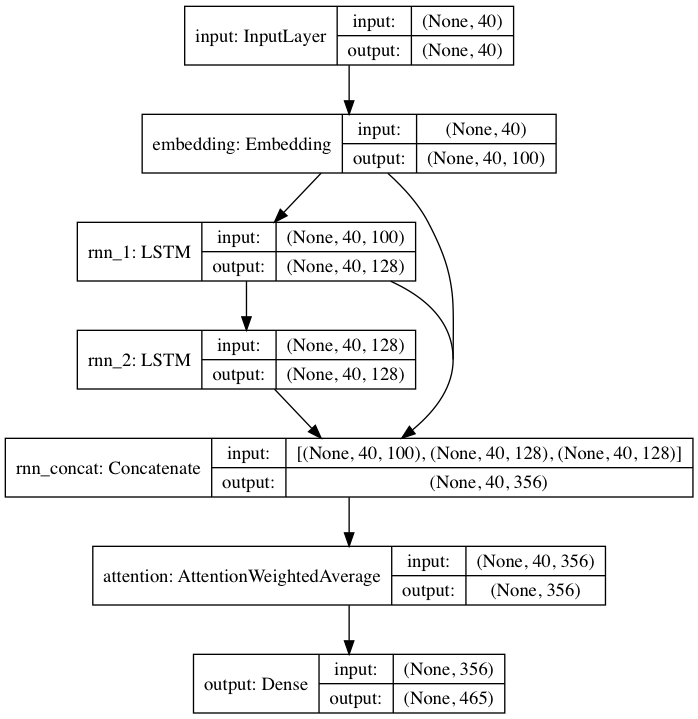
\includegraphics[scale=0.5]{default_model.png}}
    \caption{Структура модели нейронной сети в \texttt{textgenrnn}}\label{fig:default}
\end{figure}

Чтобы сгенерированные запросы были потенциально релевантны пространству поиска, сеть GPT-2 должна быть обучена на одном и том же
наборе текстов. Чтобы избежать более длительного времени обучения, но вместе с тем сохранить качество и отношение к предметной области,
для обучения рекуррентной сети была выбрана доля набора данных в размере 5\% (всего 152 документа и около 13 миллионов слов).

Кроме того, чтобы результирующие запросы не были слишком универсальными (например, содержащими только "<стоп-слова">, такие как
артикли, предлоги и другие часто используемые слова), на генератор накладываются некоторые ограничения. А именно, запрос считается
"<хорошим"> тогда и только тогда, когда он удовлетворяет одному из следующих условий:

\begin{enumerate}[1)]
    \item как минимум 1 слово встречается не более чем в 25\% от всех документов из коллекции;
    \item как минимум \(\frac{1}{3}\) слов (с округлением до ближайшего целого числа) встречается
    не более чем в 40\% от всех документов из коллекции.
\end{enumerate}

В общей сложности, в качестве эталонных было выбрано 242 запроса (на английском языке).

Примеры сгенерированных запросов:
\begin{itemize}
    \item \textit{returned earl   we had }
    \item \textit{trouble to move in oz mode which}
    \item \textit{and i don really want you to take}
    \item \textit{literature seems to be the loveliest ends }
    \item \textit{your distinction  it is i cannot as}
\end{itemize}

Как видим (по крайней мере, с точки зрения неносителя языка), запросы вполне сходны по структуре с "<настоящими"> поисковыми
запросами к системам общего назначения, таким, как Google.

Далее, в качестве эталона псевдорелевантности для обучения нейронной сети были отобраны по 10 верхних результатов по каждому из
запросов. Результаты были отранжированы согласно модифицированной формуле BM25:
\begin{equation}
    \label{eq:wbm25}
    \begin{aligned}
    \text{score}(D,Q) = w_1 \sum_{i=1}^{n} \text{IDF}(q_i) \times \\ \times \frac{f(q_i, D) \cdot (k_1 + 1)}{f(q_i, D) + k_1 \cdot \left(1 - b + b \cdot \frac{|D|}{\tilde{L}}\right)} \\
    + w_2  \sum_{i=1}^{n-1} \text{IDF}(q_i q_{i+1}) \times \\ \times \frac{f(q_i q_{i+1}, D) \cdot (k_1 + 1)}{f(q_i q_{i+1}, D) + k_1 \cdot \left(1 - b + b \cdot \frac{|D| - 1}{\tilde{L} - 1}\right)} \\
    + w_3  \sum_{i=1}^{n-2} \text{IDF}(q_i q_{i+1}q_{i+2}) \times \\ \times \frac{f(q_i q_{i+1}q_{i+2}, D) \cdot (k_1 + 1)}{f(q_i q_{i+1}q_{i+2}, D) + k_1 \cdot \left(1 - b + b \cdot \frac{|D| - 2}{\tilde{L} - 2}\right)}
    \end{aligned}
\end{equation}
где \(w_1\), \(w_2\), \(w_3\) --- весовые коэффициенты отдельных слов, биграмм и триграмм соответственно (в реализации 
использовались значения \(w_1=1\), \(w_2=10\) and \(w_3=100\)), \(f(q_1, D)\), \(f(q_1q_2, D)\) и \(f(q_1q_2q_3, D)\) --- 
частоты терминов: отдельного слова \(q_1\), биграммы \(q_1q_2\) и триграммы \(q_1q_2q_3\) соответственно (аналогично и для IDF),
 \(|D|\) --- длина документа \(D\), а \(\tilde{L}\) --- средняя длина документа в коллекции (слагаемые \(-1\) and \(-2\) 
для биграмм и триграмм соответственно были введены в связи с тем, что документ с \(N\) словами, очевидно, содержит 
\(N-1\) биграмму и \(N-2\) триграммы, поэтому "<длина"> документа окажется на один и два меньше соответственно).

Таким образом, эталонный набор данных включал в себя 2158 результатов
(это число меньше, чем $10\times242=2420$, поскольку некоторые запросы дали менее 10 результатов в целом).

\subsubsection{Генеративно-состязательная сеть}
\label{lab:gan-grammar}
GAN-сеть состояла из следующих подсетей:
\begin{itemize}
    \item подсеть $G$, использующая случайные 100-мерные векторы в качестве входных данных 
    и 32-мерные векторы результатов (метрик) запроса в качестве выходных данных;
    \item подсеть $D$, которая принимает 32-мерные векторы (как порожденные подсетью $G$, так и эталонные) и выводит скаляр, 
    который может быть интерпретирован как "<вероятность"> того, что запрос является псевдорелевантным.
\end{itemize}

В сети использовались следующие функции активации:
\begin{itemize}
    \item гиперболический тангенс
    \begin{equation}
        f(x) = \tanh x;
    \end{equation}
    \item сигмоида
    \begin{equation}
        f(x) = \frac{1}{1+e^{-x}};
    \end{equation}
    \item выпрямитель с "<протечкой"> ~\cite{DBLP:journals/corr/XuWCL15} (leaky rectified linear unit)
    \begin{equation}
        f(x) = \begin{cases}
            x, & x \geqslant 0, \\
            \alpha x, & x < 0.
        \end{cases}
    \end{equation}
\end{itemize}

Внутри подсети $G$ используется последовательное размещение слоев, как показано ниже:
\begin{itemize}
    \item входной слой с размером 100 (для случайного
    входа);
    \item слой с 256 нейронами, с использованием выпрямителя с протечкой при $\alpha = 0.2$;
    \item слой с 512 нейронами, с использованием выпрямителя с протечкой при $\alpha = 0.2$;
    \item слой с 1024 нейронами, с использованием выпрямителя с протечкой при $\alpha = 0.2$;
    \item выходной слой с размером 32, использующий гиперболический тангенс в качестве функции активации.
\end{itemize}
Внутри подсети $D$ также используется последовательное размещение слоев в следующем порядке:
\begin{itemize}
    \item входной слой с размером 32 (для подачи векторов параметров, генерируемых подсетью G);
    \item слой с 1024 нейронами, использующий ReLU с $\alpha = 0.2$;
    \item слой отсева с коэффициентом 0,3;
    \item слой с 512 нейронами, использующий ReLU с $\alpha = 0.2$;
    \item слой отсева с коэффициентом 0,3;
    \item слой с 256 нейронами, использующий ReLU с $\alpha = 0.2$;
    \item слой отсева с коэффициентом 0,3;
    \item выходной слой с размерностью 1 (скалярное значение, обозначающее оценку релевантности).
\end{itemize}

Листинг на языке Python с использованием библиотеки Keras для создания подсетей выглядит следующим образом:
\begin{lstlisting}[language=python, breaklines=true]
def get_generator(optimizer):
    generator = Sequential()
    generator.add(Dense(256, input_dim=random_dim, kernel_initializer=initializers.RandomNormal(stddev=0.02)))
    generator.add(LeakyReLU(0.2))

    generator.add(Dense(512))
    generator.add(LeakyReLU(0.2))

    generator.add(Dense(1024))
    generator.add(LeakyReLU(0.2))

    generator.add(Dense(32, activation='tanh'))
    generator.compile(loss='mse', optimizer=optimizer)
    return generator

def get_discriminator(optimizer):
    discriminator = Sequential()
    discriminator.add(Dense(1024, input_dim=32, kernel_initializer=initializers.RandomNormal(stddev=0.02)))
    discriminator.add(LeakyReLU(0.2))
    discriminator.add(Dropout(0.3))

    discriminator.add(Dense(512))
    discriminator.add(LeakyReLU(0.2))
    discriminator.add(Dropout(0.3))

    discriminator.add(Dense(256))
    discriminator.add(LeakyReLU(0.2))
    discriminator.add(Dropout(0.3))

    discriminator.add(Dense(1, activation='sigmoid'))
    discriminator.compile(loss='binary_crossentropy', optimizer=optimizer)

    return discriminator

def get_gan_network(discriminator, random_dim, generator, optimizer):
    discriminator.trainable = False
    gan_input = Input(shape=(random_dim,))
    x = generator(gan_input)
    gan_output = discriminator(x)
    gan = Model(inputs=gan_input, outputs=gan_output)
    gan.compile(loss='binary_crossentropy', optimizer=optimizer)
    return gan 
\end{lstlisting}

Для проверки сгенерированной модели был сгенерирован дополнительный набор из 51 "<хорошего"> запроса. Затем 
было использовано классическое ранжирование BM25 по формуле \eqref{eq:wbm25}, после чего из результатов поиска 
по каждому запросу были выделены верхние 10 (псевдорелевантные) и нижние 10 (псевдонерелевантные).
На следующем этапе результаты подавались через обученную модель. Некоторые результаты приведены в таблице \ref{tab1}
(средние значения $\mu$ и стандартные отклонения $\sigma$ оценок GAN-сетью для верхней и нижней групп 10), а также
на графике (рис. \ref{fig:gram-scores}), где $S_{\mathrm{ps-rel}}$ и $S_{\mathrm{ps-irr}}$ --- оценки для
псведорелевантных и псевдонерелевантных запросов соответственно.

\begin{figure}
    \centerline{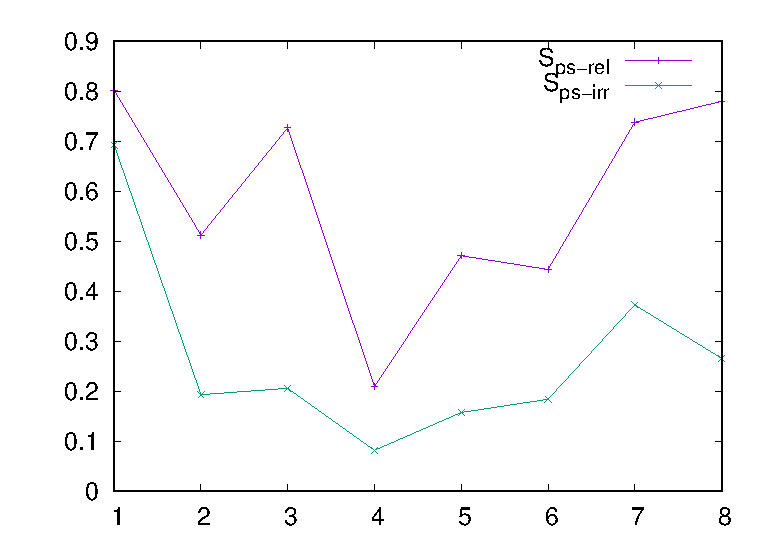
\includegraphics[scale=0.8]{311_scores.eps}}
    \caption{Оценки релевантности для модели}\label{fig:gram-scores}
\end{figure}

\begin{table}[tbp]
    \caption{Результаты поисковых запросов}
    \begin{center}
    \begin{tabular}{ccc}
    \toprule
    \textbf{Запрос}&\multicolumn{2}{c}{\textbf{Оценка релевантности}} \\
    & \textbf{\textit{Top 10}}& \textbf{\textit{Bottom 10}} \\
    \midrule
    that there were no reason on lewis& \(\mu=0.8024\) & \(\mu=0.6926\) \\
    & \(\sigma=0.1050\) & \(\sigma=0.0474\) \\
    \midrule
    i proposed marriage his visit& \(\mu=0.5127\) & \(\mu=0.1933\) \\
    & \(\sigma=0.2786\) & \(\sigma=0.0694\) \\
    \midrule
    fanny  said she& \(\mu=0.7270\) & \(\mu=0.2061\) \\
    & \(\sigma=0.2269\) & \(\sigma=0.0086\) \\
    \midrule
    published it  i think we found& \(\mu=0.2096\) & \(\mu=0.0822\) \\
    & \(\sigma=0.2077\) & \(\sigma=0.0226\) \\
    \midrule
    i shall you heart now & \(\mu=0.4713\) & \(\mu=0.1577\) \\
    & \(\sigma=0.3046\) & \(\sigma=0.0095\) \\
    \midrule
    right i had down her & \(\mu=0.4439\) & \(\mu=0.1843\) \\
    & \(\sigma=0.1391\) & \(\sigma=0.0985\) \\
    \midrule
    nice declaration  she got you  i & \(\mu=0.7382\) & \(\mu=0.3731\) \\
    & \(\sigma=0.2437\) & \(\sigma=0.0203\) \\
    \midrule
    i never moved nearer than it is & \(\mu=0.7801\) & \(\mu=0.2660\) \\
    & \(\sigma=0.1304\) & \(\sigma=0.2241\) \\
    \bottomrule
    \end{tabular}\label{tab1}
    \end{center}
\end{table}
\subsection{Модель с использованием семантической сети}

WordNet \cite{Miller95wordnet:a} --- лексическая база данных английского языка, разработанная в Принстонском университете.
Она представляет собой электронный словарь-тезаурус и набор семантических сетей для английского языка.

Словарь, представленный в WordNet, состоит из 4 семантических сетей для основных знаменательных частей речи:
существительных, глаголов, прилагательных и наречий.

Этапы применения WordNet к модели, описанной в предыдущем разделе:
\begin{enumerate}[1)]
    \item провести грамматический разбор запроса, выявить части речи, соответствующие словам;
    \item определить (хотя бы приближенно) возможную семантику слова в соответствии с контекстом;
    \item найти с использованием WordNet похожие слова (согласно метрике семантической близости);
    \item ранжировать поисковую выдачу в соответствии с семантической близостью слов и $n$-грамм для
          последующего обучения нейронной сети (с помощью классических алгоритмов либо субъективно);
    \item обучить нейросеть и провести сравнение результатов.
\end{enumerate}

Семантическая близость $n$-грамм может быть определена как среднее геометрическое коэффициентов близости отдельных слов:
\begin{equation}
    \label{eq:ngram-sim}
    \begin{aligned}
        S(u_1u_2\dots u_n, w_1w_2\dots w_n) = \left( \prod\limits_{i=1}^n {S(u_i, w_i)} \right)^{\frac1n}= \\
        = \sqrt[n]{S(u_1, w_1)S(u_1, w_2)\dots S(u_n, w_n)},
    \end{aligned}
\end{equation}
где $u_1u_2\dots u_n$ и $w_1w_2\dots w_n$ --- сравниваемые $n$-граммы (здесь мы считаем, что порядок слов имеет значение).

Формула \eqref{eq:ngram-sim} может быть продиктована следующими соображениями:
\begin{enumerate}[1)]
    \item коэффициент близости должен равняться некоторому <<среднему>> из коэффициентов близости отдельных слов;
    \item с другой стороны, наличие неподобных пар слов должно приводить к значительному (но не полному) снижению
          близости всей $n$-граммы (что позволяет отсечь, например, среднее арифметическое).
\end{enumerate}

Одним из базовых методов для выведения семантики слова в контексте (разрешения неоднозначности, англ. disambiguation)
является метод Леска \cite{10.1145/318723.318728}, разработанный инженером компании Bell Labs М. Леском в 1986 году.
Идея метода заключается в поиске значения слова в списке словарных определений с учетом контекста, где это слово использовано.
Основным критерием для выбора значения послужило следующее правило: заложенный в этом определении смысл должен был частично
совпадать со смыслом значений соседних слов в контексте.

Алгоритм Леска работает в следующей последовательности:
\begin{enumerate}[1)]
    \item На первом шаге алгоритма отделяется контекст для рассматриваемого слова --- чаще всего, не более 10 расположенных
          рядом слов.
    \item Далее, для рассматриваемого слова (или его начальной формы) ищутся все определения в некоторой базе знаний
          (например, толковом словаре, хотя данный вариант редко используется непосредственно).
    \item Затем происходит поиск слов из контекста в каждом найденном определении. Если какое-либо слово из контекста
          присутствует в определении, то данное определение получает "<балл"> --- т. е. увеличивается счетчик совпадений.
    \item Наконец, происходит ранжирование определений по значениям счетчика совпадений. Чем выше значение счетчика, тем более
          подходящим к контексту считается определение.
\end{enumerate}

Рассмотрим следующий пример: согласно Большому толковому словарю русского языка С. А. Кузнецова \cite{kuznecov2008noveishiy},
слово "<штанга"> в русском языке имеет следующие значения:
\begin{enumerate}[1)]
    \item металлический стержень, используемый как деталь во многих механизмах;
    \item боковая стойка (иногда и верхняя перекладина) футбольных, хоккейных и т.п. ворот;
    \item снаряд для занятий тяжёлой атлетикой, состоящий из металлического стержня, на концах которого укреплены
          съёмные диски различного веса.
\end{enumerate}

Теперь рассмотрим следующие предложения, содержащие слово "<штанга">:
\begin{enumerate}[1)]
    \item Троллейбусная штанга, как правило, изготовляется из металлической трубы переменного сечения.
    \item В футбольном матче между "<Спартаком"> и "<Зенитом"> форвард ленинградцев дважды поразил штангу, а защитник москвичей
          отметился голом в свои ворота.
    \item На чемпионате мира по тяжелой атлетике наш спортсмен поднял штагу рекордного веса.
\end{enumerate}

Как видим, в первом предложении присутствует слово "<металлический">, которое есть только в первом определении слова "<штанга">.
Во втором предложении такую же роль играют слова "<футбольный"> и "<ворота">, в третьем --- "<вес"> и "<тяжелая атлетика">.
Таким образом, в данном примере алгоритм работает безупречно, правильно определяя значение слова в зависимости от контекста.

Чаще, к сожалению, возникает обратная ситуация --- а именно, когда словарное определение оказывается недостаточно емким и не включает
в себя наиболее часто встречающиеся в контексте слова. Поэтому чаще применяются модификации алгоритма, основанные не только на
словарных определениях, но и на примерах употребления слов в данных значениях в контексте.

Для применения алгоритма воспользуемся методом, содержащимся непосредственно в библиотеке NLTK. Он возвращает для заданного слова
в предложении наиболее подходящий (с точки зрения алгоритма) набор синонимов, иначе --- синонимический ряд (англ. synset),
представляющий из себя слова со схожим значением, объединенные в узел семантической сети. В WordNet каждый такой набор дополнен
определением и примерами употребления слов в контексте. Слова, имеющие несколько значений, включаются в несколько синонимических рядов
(выбор между которыми в контексте заданного поискового запроса или предложения будет осуществляться с помощью алгоритма Леска)
и могут быть причислены к различным синтаксическим и лексическим классам.

Синонимические ряды, в отличие от лишенных контекста слов, уже подлежат количественной оценке схожести.

В качестве метрики семантической близости воспользуемся метрикой Ву-Палмер \cite{10.3115/981732.981751}, предложенной в 1994 году
специалистами по компьютерной лингвистике Чжибяо Ву и Мартой Палмер. Она вычисляется по следующей формуле
\begin{equation}
    \label{eq:wup-sim}
    S_{WP} = 2\times\frac{d(\mathrm{LCS}(s_1, s_2))}{d(s_1) + d(s_2)}
\end{equation}
Здесь $d(s)$ --- глубина синонимического ряда $s$ в таксономии WordNet, $\mathrm{LCS}(s_1, s_2)$ --- наиболее специфический
(то есть, наименее общий) узел (англ. least common subsumer), являющийся предком как $s_1$, так и $s_2$.

Заметим, что метрика \eqref{eq:wup-sim} определена не всегда, поскольку таксономия может не быть деревом (в общем случае, это лес),
а значит, $\mathrm{LCS}(s_1, s_2)$ для произвольных $s_1$ и $s_2$ может не существовать. Однако же, в нашем случае, поскольку мы
во всех случаях вычисляем метрику подобия между схожими словами, имеющими общего предка в таксономии.

Если метрика \eqref{eq:wup-sim} определена, то всегда $0 < S_{WP}\leqslant 1$ (заметим, что она всегда строго больше 0, поскольку
глубина корня в таксономии по определению считается равной 1).

Для некоторых частей речи в WordNet (в частности, прилагательных и наречий) таксономия не организована в виде иерархии, поэтому
вычисление $S_{WP}$ становится невозможным. Наиболее простым подходом в таком случае является назначение таким парам синонимических
рядов константной метрики, то есть, фиксированного значения $0 < \alpha < 1$ (значение 1 используется только в случае, когда $s_1=s_2$,
то есть, слово считается максимально близко семантически самому себе). В нижеописанных экспериментах используется данный подход,
применяется значение $\alpha=0{,}2$.

Далее, нам необходимо модифицировать метрики TF-IDF \eqref{eq:norm-tf} и \eqref{eq:shifted-idf} для того, чтобы они учитывали вхождение
в тексты документов не только самих слов, но и их синонимов (включая семантическую близость). Наиболее естественным для этого представляется
подход с использованием взвешенного количества слов:

\begin{equation}
    \label{eq:adjusted-word-count}
    \tilde{N}_w(d) = \sum\limits_{s\in\mathrm{Syn}(w)} N_s(d) S_{WP}(w, s)
\end{equation}
Здесь $\tilde{N}_w(d)$ --- количество вхождений слова $w$ и его синонимов (с учетом близости) в документ $d$, $\mathrm{Syn}(w)$ --- множество
синонимов слова $w$ (подразумевается, что слово считается синонимом самого себя, т.е. $w\in\mathrm{Syn}(w)$ и $S_{WP}(w, w)=1$).

Заметим, что "<количество">, определенное по формуле \eqref{eq:adjusted-word-count}, может и не быть целым числом (что очевидно следует из
определения). Однако, это не влияет на корректность вычислений метрик TF-IDF по формулам \eqref{eq:norm-tf} и \eqref{eq:shifted-idf}.

\subsubsection{Источники текстовых документов и база данных}
В рассматриваемой модели использовались те же источники (см. стр. \pageref{lab:sources-grammar}) и та же база данных (стр. \pageref{lab:db-grammar}),
что и в модели на основе грамматической структуры текстов, рассмотренной в предыдущем разделе.

\subsubsection{Генеративно-состязательная сеть}
Помимо топологии генеративно-состязательной сети, использованной в предыдущей модели (см. стр. \pageref{lab:gan-grammar}), была использована модель с
с добавлением дополнительного слоя с 2048 нейронами. Структура всей сети выглядит следующим образом:
\begin{itemize}
    \item для подсети $G$:
          \begin{itemize}
              \item входной слой с размером 100 (для случайного
                    входа);
              \item слой с 256 нейронами, с использованием выпрямителя с протечкой при $\alpha = 0.2$;
              \item слой с 512 нейронами, с использованием выпрямителя с протечкой при $\alpha = 0.2$;
              \item слой с 1024 нейронами, с использованием выпрямителя с протечкой при $\alpha = 0.2$;
              \item слой с 2048 нейронами, с использованием выпрямителя с протечкой при $\alpha = 0.2$;
              \item выходной слой с размером 32, использующий гиперболический тангенс в качестве функции активации.
          \end{itemize}
    \item для подсети $D$:
          \begin{itemize}
              \item входной слой с размером 32 (для подачи векторов параметров, генерируемых подсетью G);
              \item слой с 2048 нейронами, использующий ReLU с $\alpha = 0.2$;
              \item слой отсева с коэффициентом 0,3;
              \item слой с 1024 нейронами, использующий ReLU с $\alpha = 0.2$;
              \item слой отсева с коэффициентом 0,3;
              \item слой с 512 нейронами, использующий ReLU с $\alpha = 0.2$;
              \item слой отсева с коэффициентом 0,3;
              \item слой с 256 нейронами, использующий ReLU с $\alpha = 0.2$;
              \item слой отсева с коэффициентом 0,3;
              \item выходной слой с размерностью 1 (скалярное значение, обозначающее оценку релевантности).
          \end{itemize}
\end{itemize}

\subsubsection{Полученные результаты}
Результаты для обеих конфигураций генеративно-состязательных сетей представлены в таблицах \ref{tab2} и \ref{tab3}.
\begin{table}[tbp]
    \caption{Результаты поисковых запросов в модели с 3 слоями}
    \begin{center}
        \begin{tabular}{ccc}
            \toprule
            \textbf{Запрос}                           & \multicolumn{2}{c}{\textbf{Оценка релевантности}}                               \\
                                                      & \textbf{\textit{Top 10}}                          & \textbf{\textit{Bottom 10}} \\
            \midrule
            india  fifteen minutes more he passed     & \(\mu=0.6021\)                                    & \(\mu=0.3059\)              \\
                                                      & \(\sigma=0.2263\)                                 & \(\sigma=0.0312\)           \\
            \midrule
            that he had also seen her                 & \(\mu=0.8491\)                                    & \(\mu=0.2677\)              \\
                                                      & \(\sigma=0.0158\)                                 & \(\sigma=0.3058\)           \\
            \midrule
            more serious than by you do know          & \(\mu=0.8759\)                                    & \(\mu=0.1647\)              \\
                                                      & \(\sigma=0.0506\)                                 & \(\sigma=0.0233\)           \\
            \midrule
            answer that he asked questions to come to & \(\mu=0.8948\)                                    & \(\mu=0.8529\)              \\
                                                      & \(\sigma=0.0080\)                                 & \(\sigma=0.0506\)           \\
            \midrule
            was a bull turned from sam                & \(\mu=0.8709\)                                    & \(\mu=0.5615\)              \\
                                                      & \(\sigma=0.0355\)                                 & \(\sigma=0.3926\)           \\
            \midrule
            likely place that was with such matters   & \(\mu=0.7994\)                                    & \(\mu=0.3423\)              \\
                                                      & \(\sigma=0.1651\)                                 & \(\sigma=0.3689\)           \\
            \midrule
            and when i tried to the greatest          & \(\mu=0.9092\)                                    & \(\mu=0.8777\)              \\
                                                      & \(\sigma=0.0236\)                                 & \(\sigma=0.0165\)           \\
            \midrule
            i knew una had wept  he                   & \(\mu=0.6551\)                                    & \(\mu=0.3681\)              \\
                                                      & \(\sigma=0.1944\)                                 & \(\sigma=0.0360\)           \\
            \bottomrule
        \end{tabular}\label{tab2}
    \end{center}
\end{table}
\begin{table}[tbp]
    \caption{Результаты поисковых запросов в модели с 4 слоями}
    \begin{center}
        \begin{tabular}{ccc}
            \toprule
            \textbf{Запрос} & \multicolumn{2}{c}{\textbf{Оценка релевантности}}                               \\
                            & \textbf{\textit{Top 10}}                          & \textbf{\textit{Bottom 10}} \\
            \midrule
            then true for its sake on himself         & \(\mu=0.6028\)                                    & \(\mu=0.0888\)              \\
                                                      & \(\sigma=0.3811\)                                 & \(\sigma=0.0567\)           \\
            \midrule
            she answered   presently i said           & \(\mu=0.8736\)                                    & \(\mu=0.0272\)              \\
                                                      & \(\sigma=0.0147\)                                 & \(\sigma=0.0028\)           \\
            \midrule
            within hollow her large eyes large full   & \(\mu=0.4586\)                                    & \(\mu=0.0408\)              \\
                                                      & \(\sigma=0.4197\)                                 & \(\sigma=0.0049\)           \\
            \midrule
            how you did  i have been                  & \(\mu=0.5236\)                                    & \(\mu=0.0110\)              \\
                                                      & \(\sigma=0.4211\)                                 & \(\sigma=0.0019\)           \\
            \midrule
            other but he found his courage at least   & \(\mu=0.8612\)                                    & \(\mu=0.6925\)              \\
                                                      & \(\sigma=0.0046\)                                 & \(\sigma=0.1937\)           \\
            \midrule
            my life very that was than ever           & \(\mu=0.7160\)                                    & \(\mu=0.2305\)              \\
                                                      & \(\sigma=0.3386\)                                 & \(\sigma=0.3608\)           \\
            \midrule
            deem  remember that he was interests      & \(\mu=0.7913\)                                    & \(\mu=0.3335\)              \\
                                                      & \(\sigma=0.1954\)                                 & \(\sigma=0.2972\)           \\
            \midrule
            oh don  your true taste white             & \(\mu=0.1604\)                                    & \(\mu=0.0718\)              \\
                                                      & \(\sigma=0.1300\)                                 & \(\sigma=0.0042\)           \\
            \bottomrule
        \end{tabular}\label{tab3}
    \end{center}
\end{table}
Заметим, что при использовании обеих топологий прослеживается четкая грань между псевдорелевантными и псевдонерелевантными результатами поисковой выдачи.
Следует также заметить, что сравнение абсолютных оценок релевантности для разных запросов смысла не имеет, важны лишь относительные оценки для каждого 
конкретного запроса в отдельности (поскольку при ранжировании результатов каждый запрос обрабатывается по отдельности, а выдача ранжируется (сортируется)
в соответствии со значением оценки, которе используется лишь для определения позиции (ранга) результата в выдаче по запросу).

На основании полученных результатов мы можем сразу же выявить преимущества и недостатки модели,
основанной на WordNet, по сравнению с простейшей моделью, учитывающей лишь грамматические словоформы:
\begin{itemize}
    \item увеличился охват запросов документами, в связи с тем, что, в отличие от предыдущей модели, в рассматриваемой
          учитываются не только сами слова, входящие в запрос, но и семантически близкие им. Это в некоторых случаях позволило
          увеличить точность запросов и релевантность результатов, что показало больший разброс в поисковой выдаче и дало
          возможность продемонстрировать различия в псевдорелевантных и псевдонерелевантных результатах;
    \item с другой стороны, контекст запроса часто не позволяет однозначно определить семантику того или иного слова 
          в типологии WordNet. В частности, в ходе подготовки данных для моделей и отладки написанных программ было
          выяснено, что в ходе применения алгоритма Леска для часто распространенных английских слов I (я) и as (союз "<как">)
          в качестве синонимов часто упоминались слова indium (индий) и arsenic (мышьяк). Это связано с символами I и As для
          соответствующих химических элементов --- индия и мышьяка, которые практически во всех случаях не имели реального
          отношения к запросу;
    \item WordNet не позволяет опредлить на уровне метрики подобие некоторых частей речи (в частности, прилагательных), но применение
          константного значения для пар синонимических рядов с неопределенной метрикой нельзя считать исчерпывающим решением проблемы,
          поскольку прилагательные также могут иметь неравноценные синонимы.
\end{itemize}
В целом, WordNet является базой знаний для текстов общего назначения, поэтому ее применение к специализированным корпусам текстов 
(специализация пространства поиска) не всегда может давать лучшие результаты (поэтому перспективным представляется использование модели,
описанной в следующем разделе, поскольку она может быть обучена на исходных данных того же характера, что и входящие в пространство поиска 
(включая сами данные из пространства поиска)). Подводя итог сказанному, можем заключить, что модель с использованием WordNet имеет как
свои преимущества, так и недостатки по сравнению с простейшей моделью, однако путем грамотного и обоснованного подбора баз знаний (в частности,
таксономий типа WordNet) и настройки параметров можно добиться улучшения результатов и использования всех преимуществ WordNet (следует, однако,
заметить, что процесс этот требудет значительного объема "<ручного"> (то есть, неавтоматизируемого, требующего серьезного вмешательства человека) труда,
что не во всех случаях является лучшим решением).
\subsection{Модель с использованием векторного представления слов}
Word2vec --- общее название для совокупности моделей на основе искусственных нейронных сетей, предназначенных для получения
векторных представлений слов на естественном языке. Используется для анализа семантики естественных языков, основанный
на дистрибутивной семантике, машинном обучении и векторном представлении слов. Программное обеспечение под названием
<<Word2vec>> было разработано группой исследователей Google в 2013 году \cite{mikolov-etal-2013-linguistic,mikolov2013efficient}.
Подобные модели и инструменты разрабатывались и ранее, еще в 2000-х годах (\cite{bengio2003neural,collobert2008}),
однако первой популярной реализацией векторно-семантической модели стала именно Word2vec.

Заметим, что ошибочно называть Word2vec алгоритмом --- в совокупности реализованы два основных алгоритма обучения:
CBoW (англ. Continuous Bag of Words, <<непрерывный мешок со словами>>, англ. bag --- мультимножество)
и Skip-gram.

CBoW --- архитектура, которая предсказывает текущее слово, исходя из окружающего его контекста. С другой стороны, архитектура
типа Skip-gram действует наоборот: она использует текущее слово, чтобы предугадывать окружающие его слова.
Построение модели word2vec возможно с помощью двух данных алгоритмов.
Порядок слов контекста не оказывает влияния на результат ни в одном из этих алгоритмов.

Архитектура модели CBoW пытается предсказать текущее целевое слово (центральное слово) на основе исходных контекстных слов
(окружающих слов) \cite{kdnuggets2018cbow}.

Семейство моделей Word2Vec относится к обучению без учителя, это означает, что мы можем просто подать на вход нейросети из этого семейства
корпус без дополнительных меток или информации, и она может создавать плотные векторные представления слов (также "<вложения слов">,
англ. word embedding --- по состоянию на 2021 год, перевод этого термина на русский не устоялся) из корпуса.
Но, тем не менее, чтобы получить данные представления, потребуется использовать классификационную методологию путем обучения с учителем.
Однако, это возможно сделать с использованием лишь данных корпуса, без какой-либо вспомогательной информации.
Архитектура CBoW может быть смоделирована как модель классификации глубокого обучения, в качестве входных данных $X$ в которой берутся
контекстные слова, а объектом предсказания $Y$ служит целевое слово. Построение этой архитектуры проще, чем модели Skip-gram,
которая пытается предсказать целый ряд контекстных слов из исходного целевого слова.

С другой стороны, Skip-gram используется для предсказания контекстных слова для данного целевого слова. Фактически, это алгоритм, обратный CBoW.
Здесь целевое слово служит входом, а контекстные слова --- выходом. Поскольку существует более одного контекстного слова, которое нужно
предсказать, это несколько усложняет проблему \cite{tds2019skipgram}.

Топология сети Skip-gram, как правило состоит из входного слоя,

Следует также обратить внимание на то, что word2vec использует в своей работе простые нейронные сети, а это значит,
что для качественных результатов, получаемых при обучении данных сетей, необходимо иметь большой размер обучающей выборки ---
в данном случае, корпуса текстов.

В ходе исследования модели, основанной на семантической базе знаний WordNet, описанной в предыдущем разделе, был выявлен
фундаментальный ее недостаток --- а именно, модель довольно плохо учитывает значение слов именно в контексте области поиска
(поисковой базы данных), поскольку WordNet является базой общего назначения. Кроме того, адекватно определить семантическую
близость некоторых категорий слов невозможно путем использования только WordNet.

В противоположность вышеописанной, модель с использованием алгоритмов word2vec может обучаться на произвольном наборе текстов,
а это значит, что для обучения мы можем использовать саму поисковую базу (то есть, выборку текстов непосредственно из корпуса).

Хотя алгоритмы Word2vec не являются глубинными нейронными сетями в классическом понимании этого термина, однако, они представляют
слова в числовой форме, которая уже может быть принята к обработке сетями глубокого обучения.

Практические приложения Word2vec выходят за рамки разбора предложений в реальных текстовых документах. Данный класс алгоритмов
также может быть применен к таким разнообразным областям, как генетические последовательности, исходные коды программного обеспечения,
"<лайки"> пользователей в социальных сетях или на других подобных площадках, графы социальных сетей и другие последовательности
слов или символов, в которых можно выявить некие закономерности --- паттерны (англ. pattern --- образец).

Почему данный подход возможен при применении к столь разнообразным областям? Заметим, что мы можем представлять слова как
дискретные состояния, равно как и другие данные, упомянутые выше, а алгоритмы класса Word2vec позволяют находить переходные вероятности
между этими состояниями, то есть, насколько правдоподобно то, что слова (гены, последователи в социальных сетях и тому подобное)
будут соседствовать. Таким образом, возможны модификации алгоритмов а-ля gene2vec, like2vec и follower2vec.

Цель алгоритмов Word2vec, а равно как и их практическая польза, состоит в том, чтобы сгруппировать (кластеризовать) векторы похожих
слов или иных объектов в некоем векторном пространстве. То есть, близость обнаруживается строго математически, с использованием
определенных метрик. Word2vec генерирует векторы, которые являются распределенными числовыми представлениями словесных признаков,
таких, как контекст отдельных слов внутри определенной базы текстов. Это выполняется без вмешательства человека.

При наличии достаточного количества данных, а также примеров их использования и контекстов Word2vec может со значительной точностью
сделать предположения о значении слова, основанные на его прошлых появлениях в тексте. Эти догадки могут быть использованы для
установления связи слова с другими словами (например, термин "<мужчина"> так относится к термину "<мальчик">, как "<женщина">
к "<девочке">), либо для кластеризации документов и классификации их по темам. Эти кластеры могут служить основой для поиска (что
рассматривается в данной работе), анализа настроений и рекомендаций в таких разнообразных областях, как научные исследования,
сбор доказательств, электронная коммерция и управление взаимоотношениями с клиентами.

Выходные данные нейронной сети Word2vec представляют из себя словарь, ключами в котором являются слова (или иные рассматриваемые объекты),
а значениями --- векторы, которые можно подавать на сети глубокого обучения, либо же использовать для обнаружения связей между словами
путем простых запросов по ключу (что прежде всего и используется в данной работе).

В качестве метрики близости для слов чаще всего берется косинусная близость (англ. cosine similarity), также коэффициент
Отиаи, Отиаи --- Баркмана (\cite{10.2307/1302424,barkman1969phytosociology,Ochiai1957ZoogeographicalSO}), предложенная японским биологом
Акирой Отиаи в 1957 году, в дальнейшем обобщенная и нашедшая применение в разнообразных приложениях и за рамками биологии.

Как известно, в евклидовом пространстве косинус (неориентированного) угла между векторами $a$ и $b$ определяется по следующей формуле:
\begin{equation}
    \cos\varphi = \frac{a\cdot b}{||a||\ ||b||}
\end{equation}
Здесь $a\cdot b$ --- скалярное произведение векторов $a$ и $b$:
\begin{equation}
    a\cdot b = \sum\limits_{i=1}^n a_i b_i,
\end{equation}
а $||a||$ --- норма вектора $a$:
\begin{equation}
    ||a||=\sqrt{\sum\limits_{i=1}^n a_i^2}
\end{equation}

Значение косинуса, согласно неравенству Коши --- Буняковского --- Шварца \cite{bhlitem176592}, может изменяться от -1
(соответствует значению $\varphi=180^{\circ}$, или $\pi$ радианов) до 1 (соответствует $\varphi=0$). Значение 0, соответствующее
$\varphi=90^{\circ}=\frac\pi2$ радианам, обозначает ортогональность векторов.

Данное значение $\cos\varphi$ используется в качестве метрики близости между векторами, то есть, и между соответствующими им словами:
1 обозначает полное совпадение векторов и слов, $-1$ --- абсолютное их различие (слова являются антонимами в модели), наконец, значение,
равное 0, показывает несвязанность (ортогональность) понятий согласно критериям модели.

Например, согласно одной из моделей Word2vec, приведенной в \cite{pathmind2021}, слова, наиболее схожие по этой метрике со словом
Sweden (Швеция), представлены в таблице \ref{tab4} (за исключением самого слова Sweden, коэффициент схожести которого с самим собой равен 1).
Как видим, в порядке убывания близости представлены названия скандинавских, затем прочих развитых североевропейских стран.

\begin{table}[tbp]
    \caption{Схожесть слов со словом Sweden}
    \begin{center}
        \begin{tabular}{rr}
            \toprule
            \textbf{Слово} & \textbf{Близость} \\
            \midrule
            Norway         & 0.760124          \\
            \midrule
            Denmark        & 0.715460          \\
            \midrule
            Finland        & 0.620022          \\
            \midrule
            Switzerland    & 0.588132          \\
            \midrule
            Belgium        & 0.585835          \\
            \midrule
            Netherlands    & 0.584631          \\
            \midrule
            Iceland        & 0.562368          \\
            \midrule
            Estonia        & 0.547621          \\
            \midrule
            Slovenia       & 0.531408          \\
            \bottomrule
        \end{tabular}\label{tab4}
    \end{center}
\end{table}

Для проектирования модели Word2vec была выбрана библиотека GenSim \cite{rehurek_lrec}, поскольку алгоритмы, реализующие
данную архитектуру, отсутствуют в NLTK. Однако же, это никоим образом не влияет на производительность и совместимость модулей,
поскольку поисковая часть независима от модуля определения семантической близости.

Модель Word2vec была обучена на 5\% поисковой базы (брался каждый 20-й документ из 3036 имеющихся). Заметим, однако, что точность
определения семантической близости для слов, редко встречающихся в корпусе текстов для обучения сети, может быть довольно низкой:
в частности, в вышеописанной сети словом, наиболее близким к имени Helena (Елена), оказалось слово secretary (секретарь), с коэффициентом
Отиаи --- Баркмана, равным приблизительно 0,87087. Это, в частности, связано с тем, что вариант написания имени Helena был малопопулярен
в Великобритании 2-й половины 19-го столетия (основу поисковой базы составляют преимущественно тексты, написанные в данное время),
значительно более популярным было написание Helen либо Ellen \cite{helen1850, helen1900}.

Параметры обучения модели следующие:
\begin{itemize}
    \item размерность векторов для представления слов была выбрана равной 100;
    \item размер "<окна">, в рамках которого слова считаются соседними, был равен 5 словам;
    \item минимальное количество вхождений слова в текст (начиная с которого, слово считается учитываемым моделью) было равно 1 
          (то есть, учитывались все слова без исключения);
    \item наконец, количество потоков для параллельного обучения было выбрано равным 16 (оптимальное значение для машины, 
          на которой проводилось обучение).
\end{itemize}

Общий объем обучающей выборки составил порядка 550 тысяч предложений. В вышеописанных условиях процесс обучения занимает
время порядка нескольких минут (на машине с процессором Ryzen 9 3950X в операционной системе Linux).

Архитектура генеративно-состязательных сетей, базы данных и других модулей полностью совпадают с рассмотренными в предыдущем разделе,
изменилась лишь методика подсчета коэффициентов семантической близости (использовалась 4-слойная модель GAN).

Для обучения генеративно-состязательной сети был сгенерирован и подобран набор из 320 поисковых запросов.

Результаты по некоторым тестовым запросам представлены в таблице \ref{tab5} % TODO: график

\begin{table}[tbp]
    \caption{Результаты поисковых запросов в модели без ограничений на количество документов в выдаче}
    \begin{center}
        \begin{tabular}{ccc}
            \toprule
            \textbf{Запрос} & \multicolumn{2}{c}{\textbf{Оценка релевантности}}                               \\
                            & \textbf{\textit{Top 10}}                          & \textbf{\textit{Bottom 10}} \\
            \midrule
            readers of you in lady byron on           & \(\mu=0.9032\)                                    & \(\mu=0.8968\)              \\
                                                      & \(\sigma=0.0011\)                                 & \(\sigma=0.0029\)           \\
            \midrule
            bowl or in their service  now then        & \(\mu=0.8965\)                                    & \(\mu=0.8912\)              \\
                                                      & \(\sigma=0.0018\)                                 & \(\sigma=0.0037\)           \\
            \midrule
            are about among the fourth the two        & \(\mu=0.9111\)                                    & \(\mu=0.8981\)              \\
                                                      & \(\sigma=0.0040\)                                 & \(\sigma=0.0011\)           \\
            \midrule
            i can do as the minutes of old            & \(\mu=0.8859\)                                    & \(\mu=0.8898\)              \\
                                                      & \(\sigma=0.0034\)                                 & \(\sigma=0.0056\)           \\
            \midrule
            tom twice caught a beautiful picture      & \(\mu=0.8837\)                                    & \(\mu=0.8717\)              \\
                                                      & \(\sigma=0.0021\)                                 & \(\sigma=0.0077\)           \\
            \midrule
            races  rudimentary organs on              & \(\mu=0.0023\)                                    & \(\mu=0.0014\)              \\
                                                      & \(\sigma=0.0028\)                                 & \(\sigma=0.0002\)           \\
            \midrule
            take young men of made the                & \(\mu=0.8974\)                                    & \(\mu=0.8934\)              \\
                                                      & \(\sigma=0.0012\)                                 & \(\sigma=0.0008\)           \\
            \midrule
            will begin to at court east wind the      & \(\mu=0.8966\)                                    & \(\mu=0.8897\)              \\
                                                      & \(\sigma=0.0049\)                                 & \(\sigma=0.0029\)           \\
            \bottomrule
        \end{tabular}\label{tab5}
    \end{center}
\end{table}

Как видим, для некоторых запросов результаты для верхней и нижней десяток практически неразличимы (статистически незначимы).
Это обусловлено в основном двумя (в некотором смысле взаимодополняющими) причинами, а именно:
\begin{enumerate}[1)]
    \item для многих запросов в выдачу попали почти все документы (вплоть до 2900--3000 из 3036), при этом запросы содержали в основном 
          широкоупотребительные слова, частота встречаемости которых в документах практически не различается, а значит, и значения оценки BM25,
          на которых обучалась модель, будут лишь несущественно отличны. В таком случае релевантность всех результатов будет приблизительно 
          одинаковой, к тому же, говорить о практической значимости такого ранжирования по большому счету не имеет смысла в связи с тем,
          что подобные поисковые запросы слишком малоинформативны;
    \item с другой стороны, для некоторых запросов область результатов, наоборот, оказалась слишком узкой, в некоторых случаях документов,
          попавших в выдачу, оказалось менее 20, то есть множества top-10 и bottom-10 и вовсе перекрывались. В таких случаях, поскольку
          количество документов, удовлетворяющих запросу, достаточно мало, проблема релевантности не стоит остро, поскольку пользователь,
          подающий запрос к поисковой системе, в подобных случаях может перебрать результаты напрямую с минимальными трудозатратами.
\end{enumerate}

В связи с вышеописанными причинами, для устранения подобных "<патологических"> примеров, введем дополнительный критерий фильтрации тестовых
запросов:
\begin{itemize}
    \item будем считать запрос пригодным для тестирования, если количество документов, содержащих все слова из запроса (или семантически
          близкие им), содержит не менее 10, но не более 40 процентов от общего количества документов в корпусе (в нашем случае, от 304 до 1214
          из 3036).
\end{itemize}

Результаты с фильтрацией по данному принципу представлены в \ref{tab6} % TODO: график
\begin{table}[tbp]
    \caption{Результаты поисковых запросов в модели с примененными ограничениями}
    \begin{center}
        \begin{tabular}{ccc}
            \toprule
            \textbf{Запрос} & \multicolumn{2}{c}{\textbf{Оценка релевантности}}                               \\
                            & \textbf{\textit{Top 10}}                          & \textbf{\textit{Bottom 10}} \\
            \midrule
            an necessity   he did not                 & \(\mu=0.8746\)                                    & \(\mu=0.0158\)              \\
                                                      & \(\sigma=0.0573\)                                 & \(\sigma=0.0294\)           \\
            \midrule
            for sir henry james  if i                 & \(\mu=0.8935\)                                    & \(\mu=0.3722\)              \\
                                                      & \(\sigma=0.0025\)                                 & \(\sigma=0.3712\)           \\
            \midrule
            has told arthur he had an unusual movement& \(\mu=0.3169\)                                    & \(\mu=0.1191\)              \\
                                                      & \(\sigma=0.3300\)                                 & \(\sigma=0.0811\)           \\
            \midrule
            as und you be fed for us is               & \(\mu=0.8673\)                                    & \(\mu=0.3558\)              \\
                                                      & \(\sigma=0.0554\)                                 & \(\sigma=0.3477\)           \\
            \midrule
            egyptians back      why                   & \(\mu=0.0074\)                                    & \(\mu=0.0007\)              \\
                                                      & \(\sigma=0.0185\)                                 & \(\sigma<0.0001\)           \\
            \midrule
            byron works   he handed it with           & \(\mu=0.8973\)                                    & \(\mu=0.7742\)              \\
                                                      & \(\sigma=0.0017\)                                 & \(\sigma=0.2588\)           \\
            \midrule
            one when charlotte told her story she found& \(\mu=0.8703\)                                    & \(\mu=0.1288\)              \\
                                                      & \(\sigma=0.0664\)                                 & \(\sigma=0.1885\)           \\
            \midrule
            deane looked at him    you                & \(\mu=0.8943\)                                    & \(\mu=0.3500\)              \\
                                                      & \(\sigma=0.0037\)                                 & \(\sigma=0.3786\)           \\
            \bottomrule
        \end{tabular}\label{tab6}
    \end{center}
\end{table}
\printbibliography[title={Список использованных источников},category=cited]
\printbibliography[title={Непроцитированные источники (должно быть пусто)},notcategory=cited]
\end{document}